\documentclass[tikz,10pt,border=2mm]{standalone}
\usepackage{mathpazo,zi4,calligra,xcolor,structmech,siunitx}
\usetikzlibrary{backgrounds}
\definecolor{0066CC}{RGB}{0,102,204}
\definecolor{CC0066}{RGB}{204,0,102}
\definecolor{00CC66}{RGB}{0,204,102}
\definecolor{CC6600}{RGB}{204,102,0}
\definecolor{DDDDDD}{RGB}{204,204,204}
\begin{document}
\scriptsize
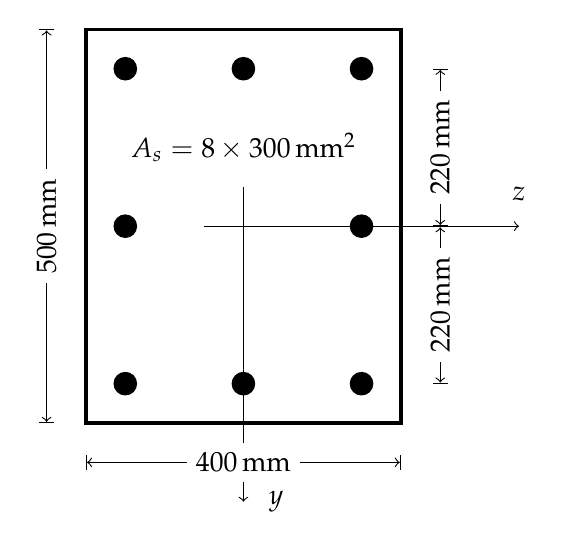
\begin{tikzpicture}
\setstructmech{linewidth=.8pt}
\draw[very thick](-2,-2.5)rectangle(2,2.5);
\draw[->](-.5,0)--++(4,0)node[above=2mm]{$z$};
\draw[->](0,.5)--++(0,-4)node[right=2mm]{$y$};
\draw[|<->|](-2.5,-2.5)--++(0,5)node[rotate=90,fill=white,midway]{\SI{500}{\milli\metre}};
\draw[|<->|](-2,-3)--++(4,0)node[fill=white,midway]{\SI{400}{\milli\metre}};
\draw[|<->|](2.5,-2)--++(0,2)node[rotate=90,fill=white,midway]{\SI{220}{\milli\metre}};
\draw[|<->|](2.5,0)--++(0,2)node[rotate=90,fill=white,midway]{\SI{220}{\milli\metre}};
\node[inner sep=0,minimum size=3mm,circle,fill=black]at(-1.5,-2){};
\node[inner sep=0,minimum size=3mm,circle,fill=black]at(0,-2){};
\node[inner sep=0,minimum size=3mm,circle,fill=black]at(1.5,-2){};
\node[inner sep=0,minimum size=3mm,circle,fill=black]at(-1.5,2){};
\node[inner sep=0,minimum size=3mm,circle,fill=black]at(0,2){};
\node[inner sep=0,minimum size=3mm,circle,fill=black]at(1.5,2){};
\node[inner sep=0,minimum size=3mm,circle,fill=black]at(-1.5,0){};
\node[inner sep=0,minimum size=3mm,circle,fill=black]at(1.5,0){};
\node at(0,1){$A_s=8\times\SI{300}{\milli\metre^2}$};
\end{tikzpicture}
\end{document}